
%%
%%  Beam Loading Paper '17
%% ***************************
%%  Veronica K. Berglyd Olsen
%%

\documentclass[aps,prstab,reprint,amsmath,amssymb,groupedaddress]{revtex4-1}
\bibliographystyle{apsrev4-1}

\usepackage{hyperref}
\hypersetup{colorlinks=true, citecolor=blue, urlcolor=blue, linkcolor=blue}

\usepackage{graphicx}


% Custom Commands
%*****************

% Text
%~ \newcommand{\eq}[1]{Eq. \ref{#1}}
%~ \newcommand{\fig}[1]{Fig. \ref{#1}}
%~ \newcommand{\tbl}[1]{Table \ref{#1}}

% Math
\newcommand{\unit}[1]{\,\mathrm{#1}}
\newcommand{\funit}[2]{\,\mathrm{#1}/\mathrm{#2}}
\newcommand{\mexp}[1]{\mathrm{e}^{#1}}
\newcommand{\nexp}[1]{\times 10^{#1}}

% ******************************************************************************************************************** %
\begin{document}
% ******************************************************************************************************************** %

%~ Eric's Comments
%~ Sec N: Beam loading [in this section we describe the interesting physics, based on a single parameters set]
%~ - describe proton beam wake structure [similar to that of a modulated proton beam] (simulation results to show:
%~   unloaded wake)
%~ - by varying the current of the electron beam, the electron beam may load the wake and the longitudinal field can be
%~   flatten and energy spread reduced [well known result, Tzoufras] 
%~ - the electron beam blows out the remaining plasma electrons. The transverse fields are dominated by the linear
%~   focusing fields originating from the ion background, leading to emittance preservation of the part of the electron
%~   beam inside the bubble [loading of a quasi-linear wake, and still get emittance preservation: this is new]
%~   (simulation results to show: loaded wake, with bubble - many different aspects of this, trans., long. field,
%~   electron densities etc. )
%~ - the acceleration and the transverse emittance stable on long timescales (simulation results to show: transverse and
%~   longitudinal phase spaces, space long simulation)
%~ - in this regime, emittance preservation is robustness to drive-witness offset [this is new] (simulation results to
%~   show: transverse and longitudinal phase spaces, long offset simulation)
%~ Sec N+1: Parameter optimization, or, parameter scaling [in this section we describe how to optimize the electron
%~ beam, and preferably some scalings]
%~ - how to select electron beam parameters:
%~ - longitudinal parameters bunch length and current (simulations results to show: overloaded/underloaded cases)
%~ - transverse parameters of electron emittance / matching [too large, outside bubble.  Do we see increased head
%~   erosion -> faster decay]?  (simulations results to show: evolution of high emittance vs low emittance cases)
%~ (- plasma density?)


%~ Patric's Comments
%~ - Self-modulation as a driver
%~ - SM does not reach blow out
%~ - SM does not preserve emittance and produces large energy spread and parameters may evolve along the accelerator,
%~   not desirable
%~ - Beam loading for narrow energy spread
%~ - Beam loading in linear regime (old papers from SLAC in the 80's, then Katsouleas for PWFA) and nonlinear regime
%~   (Tzoufras) well know
%~ - Propose "new regime" in the SM case, beam loading and blowout to get emittance preservation
%~ - Limitation as for PWFA driver, must use some of the W bunch to reach the blowout, it is kind of like the early SLAC
%~   experiments (84GeV) where the W-bunch is like the D-bunch in these experiments, but in a plasma prepared by the p+
%~   bunch and the SM
%~ - maybe also something about the fact that 200pC in a 60µm bunch corresponds to a 1kA current, much larger than the
%~   p+ bunch current, because of the fact that the wakefields are driven my multiple bunches?
%~ As for N+2, I am a firm supporter of on-axis injection ... and most of the issue with that has to do with the plasma
%~ ramp, otherwise it would be a non-issue (assuming of course that one can split the plasma in two sections). It is in
%~ itself a topic of research, so I think we can only state a few things ...


\title{Emittance preservation of an electron beam in a loaded quasi-linear plasma wakefield}

\author{Veronica K. Berglyd Olsen}
\email[]{v.k.b.olsen@cern.ch}

\author{Erik Adli}
\affiliation{University of Oslo, Oslo, Norway}

\author{Patric Muggli}
\affiliation{Max Planck Institute for Physics, Munich, Germany}
\affiliation{CERN, Geneva, Switzerland}

\date{\today}

\begin{abstract}
We investigate beam loading and emittance preservation for a high-charge electron beam being accelerated in quasi-linear
plasma wakefield driven by a short proton beam. The structure of the wakefield is similar to that of a long, modulated
proton beam, such as the one being studied by AWAKE.  We show that by exploiting two well known effects, full blow out
of plasma electrons by the accelerated beam, and beam loading of the wake field, the electron beam can be accelerated
without significant emittance growth.
\end{abstract}

\maketitle

% ******************************************************************************************************************** %
\section[\label{S:I}]{Introduction}
% interested from SMI/AWAKE
% requirements for AWAKE Run 2
% ******************************************************************************************************************** %

Beam driven plasma wakefield accelerators have the potential to offer compact linear accelerators with high energy
gradients, and have been of interest for several decades \cite{chen:1985}. A relativist beam travelling through a plasma
excites a strong longitudinal e-field that can be loaded by a trailing witness beam. With optimal beam loading, increase
in energy spread can be kept to a minimum. Acceleration of an electron withness beam by an electron drive beam has been
demonstrated experimentally \cite{rosenzweig:1988, blumenfeld:2007, kallos:2008} in the past. AWAKE at CERN is a proof
of concept proton driven plasma wakefield accelerator experiment \cite{awake_collaboration:2014}.

A major challenge with plasma wakefield accelerators is, however, to produce an accelerated beam while keeping growth in
energy spread and emittance as low as possible. In the well described linear case where the beam density $n_{b}$ is much
smaller than the plasma density $n_{0}$, the non-linear transverse wakefields cause emittance growth of the accelerated
beam. A finite length beam will also see a transversely varying accelerating field causing increasing energy spread
\cite{katsouleas:1987}. In the non-linear regime, where $n_{b} > n_{0}$, the drive beam sees a constant transverse field
due to a bubble forming in the plasma behind the drive beam. The bubble is formed by the transverse oscillations of the
plasma electrons in the wake of the drive beam, forming a sheet around an evacuated area. The ions, assumed stationary,
form an ion channel creating a focusing force that varies linearly with radius. This
produces an axially symmetric focusing force \cite{lu:2006-1, lu:2006}.
%~ This effect also avoids the issue of increasing energy spread due to transverse beam loading. Increase in energy spread
%~ is still dependent on beam loading $E_{z}$.
%~ Ideal beam loading can be achieved by specially shaped beams that optimally flattens the field
%~ \cite{katsouleas:1987, tzoufras:2009}, but this is difficult experimentally and is not a topic explored in this paper.

% ******************************************************************************************************************** %
\subsection[\label{S:I:SMI}]{Self-modulation as a Driver}
%~ Patric's Comments
%~ - Self-modulation as a driver
%~ - SM does not reach blow out
%~ - SM does not preserve emittance and produces large energy spread and parameters may evolve along the accelerator,
%~   not desirable
% ******************************************************************************************************************** %

A train of electron drive bunches with a separation $\lambda_{pe}$ and a length $l_{b} \ll \lambda_{pe}$, where
%~ \begin{align}
    %~ \lambda_{p} = 2\pi\frac{c}{\omega_{pe}} \label{EQ:LambdaP}
%~ \end{align}
%~ and
%~ \begin{align}
    %~ \omega_{pe} = \sqrt{\frac{n_{0} e^{2}}{m_{e} \epsilon_{0}}}, \label{EQ:OmegaP}
%~ \end{align}
$\lambda_{p} = 2\pi c/\omega_{pe}$ and $\omega_{pe} = (n_{0} e^{2} / m_{e} \epsilon_{0})^{1/2}$,
will produce a field $E_{z}$ that increases for each drive bunch \cite{chen:1985}. A tailing witness beam loading the
peak accelerating phase of this field will gain energy from the wakefield from all of the drive bunches. Acceleration of
an electron witness beam driven by two electron drive beams was demonstrated at Brookhaven National Laboratory
\cite{muggli:2011}.

The energy carried by electron drive bunches used in previous experiments were typically small, on the order of
$100\unit{J}$, and the propagation length typically $<1\unit{m}$ \cite{blumenfeld:2007,caldwell:2009}. De-phasing of the
witness beam relative to the drive beam, caused by loss of energy in the drive beam and gain of energy in the witness
beam, limits the effective length of a plasma accelerator stage. Proton drive beams available at CERN carry
significantly more energy, $19\unit{kJ}$ for the SPS beam \cite{gschwendtner:2016}, allowing for longer accelerator
stages. However, the SPS beam is orders of magnitude longer than the plasma wavelengths needed for such applications.
This issue is resolved by letting the proton beam undergo self-modulation before injecting the witness beam into one of
the buckets in the modulated structure. This self-modulation instability is caused by the transverse fields generated by
the beam acting upon the beam itself, causing regions of the beam to rapidly defocus \cite{kumar:2010}. The modulation
frequency is close to that of the plasma, and leaves a train of proton bunches along the beam axis with a surrounding
halo.

% ******************************************************************************************************************** %
\subsection[\label{S:I:AWAKE}]{AWAKE Run 2}
% ******************************************************************************************************************** %

%~ The first run of the experiment is set up with a $10\unit{m}$ rubidium vapour cell.
%~ The rubidium vapour is
%~ ionised by a $780\unit{nm}$, $4.5\unit{TW}$ peak power laser with a pulse length of $100−120\unit{fs}$.
The AWAKE experiment, currently in its first stages of operation at CERN, uses the SPS beam at $400\unit{GeV}$ as its
driver, and a nominal plasma density $7\nexp{14}\unit{cm}^{-3}$ \cite{gschwendtner:2016}. This plasma density
corresponds to a plasma wavelength $\lambda_{pe} = 1.26\unit{mm}$. The plasma density is matched to the SPS proton beam
such that $k_{pe}\sigma_{r} = 1$ where $k_{pe} = 2\pi/\lambda_{pe}$ is the plasma wave number. The aim of the first
phase of Run 1 of the experiment is to demonstrate self-modulation of the proton beam, and in 2018 to sample the
wakefield with a long electron beam. The study presented here is for Run 2 \cite{adli:2016}, which aims to demonstrate
acceleration of a short electron beam to high energy with a minimal increase in emittance and energy spread.

\begin{figure}[hbt]
    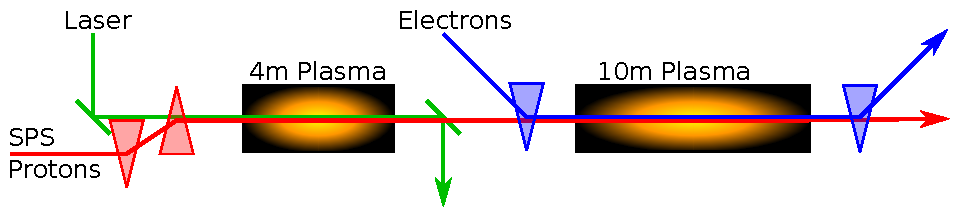
\includegraphics[width=0.99\linewidth,trim={1mm 2mm 1mm 2mm},clip]{figures/figAWAKE}
    \caption{\label{Fig:AWAKER2} A simplified illustration of the experimental setup for AWAKE Run 2. The SPS proton
        beam undergoes self-modulation in the first $4\unit{m}$ plasma cell. The electron witness beam is injected in
        one of the buckets, and undergoes acceleration in the second plasma cell \cite{berglyd_olsen:2015, adli:2016}.}
\end{figure}

The preliminary design of the second run proposes to use two plasma sections, illustrated in figure \ref{Fig:AWAKER2}.
The first section of $4\unit{m}$ is the self-modulation stage where the proton beam undergoes self-modulation without
the electron beam present. The electron witness beam will be injected into the modulated proton beam before stage two,
where acceleration will occur.
%~ As the $E_z$-field will decrease due to the gap between the two cells, it is desirable to
%~ keep this as short as possible.

With this experimental design the self-modulated proton beam does not produce a non-linear wakefield, and not all plasma
electrons are therefore evacuated. The result is that the focusing force will not increase linearly with radius. The
small size of the accelerating structure produced by the self-modulated beam also put constraints on the size of the
electron witness beam, and thus its charge and current, if we wish to prevent large energy spread. By matching the
transverse size to a practical emittance and the plasma density, we prevent large amplitude oscillations which may cause
additional growth in energy spread as well as in emittance.

The key idea in this paper is that while the proton beam wake is not fully blown-out leading to non-linear focusing
forces, the electron beam, if intense enough, may load the field and at the same time create its own ion bubble. As will
be shown, exploiting these two well known effect, the electron beam can be accelerated, for long distances, without
significant emittance growth.

%~ The beam matching relation is given by
%~ \begin{align}
    %~ \beta = \frac{\sigma_r^2}{\epsilon_g} = \frac{\lambda_pe}{2\pi}\sqrt{2\gamma_{rel}}, \label{EQ:Matched}
%~ \end{align}
%~ where $\lambda_{p}$ is the plasma wavelength. For a reasonable initial emittance of $2\unit{\mu m}$, this corresponds to
%~ a $\sigma_{r}$ of $5.25\unit{\mu m}$ -- a very narrow bunch compared to the drive beam $\sigma_{r} = 200\unit{\mu m}$.
%~ The charge density of this compact witness bunch reaches that of the plasma density at only a few $\unit{pC}$, but
%~ reaches optimal beam loading at around $1-200\unit{pC}$. The implication here being that the witness bunch produces its
%~ own non-linear wakefield already at the head of the bunch. The majority of the electrons within it will therefore see a
%~ linear focusing force preventing the bulk of the beam from undergoing emittance growth.

% ******************************************************************************************************************** %
\section[\label{S:M}]{Method}
%- explain analogy of short-bunch, SMI case, by referring to earlier Veronica-papers
%- simulation setup PIC/quickpic OS
% ******************************************************************************************************************** %

The main focus of this study has been on the beam loading of the electron beam. In order to eliminate other factors
that may affect this, we have tried several approaches to create a stable drive beam structure based on previous self-
modulation studies.

Our first approach was to use a pre-modulated, short proton beam with similar structure to the one produced by the
self-modulation of the SPS beam in AWAKE. These studies were done using the full PIC code Osiris \cite{fonseca:2002}
using 2D cylindrical-symmetric simulations \cite{berglyd_olsen:2015, berglyd_olsen:2016}.

%~ In order to evaluate the quality of the accelerated bunch it was also necessary to study emittance evolution. However,
%~ full PIC codes are vulnerable to numerical growth of emittance caused by the ``numerical Cherenkov effect''
%~ \cite{godfrey:1974}. This is a know issue with the Yee EMF solver which causes the phase velocity of electromagnetic
%~ fields to be lower than $c$ while the beam moves very close to $c$. The effect can be mitigated somewhat by replacing
%~ the Yee solver with a solver designed by Lehe \cite{lehe:2013}. Our simulations showed that this numerical effect is
%~ still prominent in the high density regions of our very compact electron bunch, making it difficult to distinguish
%~ emittance growth from the physics from that originating from numerical error.

In order to study the witness beam emittance evolution we turned to the recently released open source version of
QuickPIC developed by UCLA. QuickPIC is a fully relativistic 3D quasi-static PIC code \cite{huang:2006, an:2013}.
Since QuickPIC is a quasi-static code, it does not suffer from the numerical Cherenkov effect that full PIC codes do
\cite{godfrey:1974,lehe:2013}, it is well suited to study emittance preservation.

% ******************************************************************************************************************** %
\subsection[\label{S:M:Setup}]{Drive Beam Parameters}
%~ Patric's Comments
%~ - Self-modulation as a driver
%~ - SM does not reach blow out
%~ - SM does not preserve emittance and produces large energy spread and parameters may evolve along the accelerator,
%~   not desirable
% ******************************************************************************************************************** %

In these simulations we use a single proton drive beam that sets up a wakefield comparable to that which we expect to
see from the self-modulated SPS beam in the second plasma cell of AWAKE Run 2 (Figure \ref{Fig:AWAKER2}). When the
initial SPS beam containing $3\nexp{11}$ protons \cite{gschwendtner:2016} enters the second plasma cell the peak $E_{z}$
field is expected to be $500-600\funit{MV}{m}$. As the baseline AWAKE drive beam current is insufficient to reach the
non-linear regime and produce a plasma bubble, the plasma electrons are only depleted to around $65\%$ of nominal plasma
density at the point where we inject the electron beam \cite{awake_collaboration:2016}. These conditions are replicated
in our simulations using a single proton beam of $1.46\nexp{10}$ protons, or $2.34\unit{nC}$ and $7\unit{kA}$.

The peak density of the simulation drive beam is $0.83\cdot n_{0}$, producing a quasi-linear wakefield. The single bunch
setup uses the baseline proton energy $W_{pb} = 400\unit{GeV}$ and transverse size $\sigma_{r} = 200\unit{\mu m}$. We
set the length of the drive beam to $\sigma_{z} = 40\unit{\mu m}$. In order to create a stable environment to study the
evolution of the witness beam we prevented the proton beam from evolving radially by increasing the particle mass by a
factor of $1\mexp{6}$. We are not considering the evolution of the proton beam itself in this study.

% ******************************************************************************************************************** %
\subsection[\label{S:M:Setup}]{Witness Beam Parameters}
% ******************************************************************************************************************** %

The witness beam in our simulation differs from AWAKE baseline parameters on several key points. Initial beam energy is
set such that $\gamma_{eb} = \gamma_{pb} = 426.3$. This was done to eliminate the problem of initial de-phasing of the
witness beam. Beam loading of a short witness beam is sensitive to its position relative to the field
\cite{tzoufras:2009}. The relative drift causing the de-phasing $\Delta\xi \propto \gamma^{-2}$. By simply matching the
initial $\gamma$ values we eliminate this effect entirely, but a lower initial value is likely to be sufficient
\cite{berglyd_olsen:2015}.

In these 3D simulations we have used a matched beam for an initial emittance of $2\unit{\mu m}$, corresponding to a
$\sigma_{r}$ of $5.25\unit{\mu m}$. The beam matching relation is given by
\begin{align}
    \beta = \frac{\sigma_r^2}{\epsilon_g} = \frac{\lambda_pe}{2\pi}\sqrt{2\gamma_{rel}}, \label{EQ:Matched}
\end{align}
where $\lambda_{p}$ is the plasma wavelength. This is a very narrow beam compared to the drive beam
$\sigma_{r} = 200\unit{\mu m}$. The charge density of this compact witness beam reaches that of the plasma density at
only a few $\unit{pC}$, but reaches optimal beam loading at around $1-200\unit{pC}$. The implication here being that the
witness beam produces its own non-linear wakefield already at the head of the beam. The majority of the electrons
within it will therefore see a linear focusing force preventing the bulk of the beam from undergoing emittance growth.

The relatively small size of the witness beam compared to the proton beam put some restrictions on the transverse
resolution of the witness beam. We used a transverse grid cell size of $1.17\unit{\mu m}$, and $2.34\unit{\mu m}$ for
the longitudinal grid cells. The witness beam was simulated with $16.8\unit{M}$ non-weighted particles.

% ******************************************************************************************************************** %
\section[\label{S:BL}]{Beam Loading}
%~ Eric's Comments
%~ Sec N: Beam loading [in this section we describe the interesting physics, based on a single parameters set]
%~
%~ Patric's Comments
%~ - Beam loading for narrow energy spread
%~ - Beam loading in linear regime (old papers from SLAC in the 80's, then Katsouleas for PWFA) and nonlinear regime
%~   (Tzoufras) well know
%~ - Propose "new regime" in the SM case, beam loading and blowout to get emittance preservation
%~ - Limitation as for PWFA driver, must use some of the W bunch to reach the blowout, it is kind of like the early SLAC
%~   experiments (84GeV) where the W-bunch is like the D-bunch in these experiments, but in a plasma prepared by the p+
%~   bunch and the SM
%~ - maybe also something about the fact that 200pC in a 60µm bunch corresponds to a 1kA current, much larger than the
%~   p+ bunch current, because of the fact that the wakefields are driven my multiple bunches?
% ******************************************************************************************************************** %

\begin{figure}[hbt]
    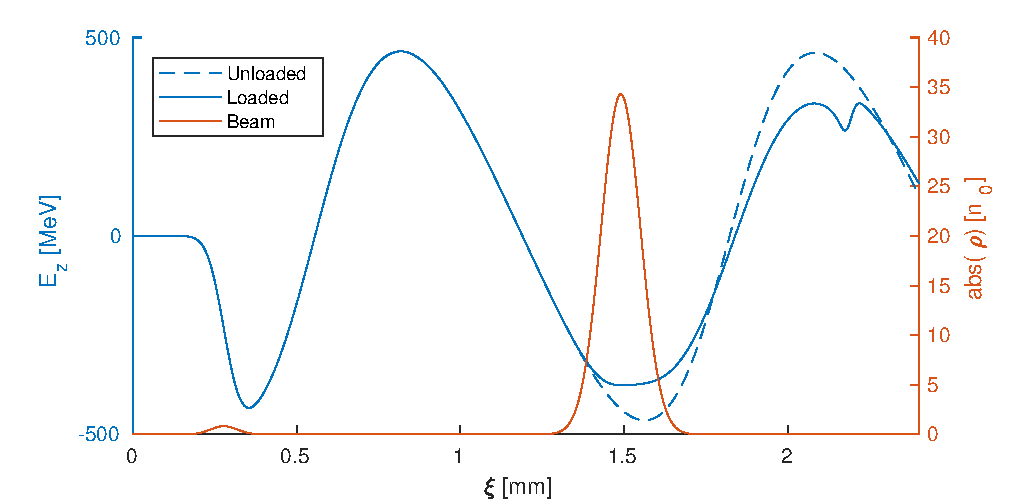
\includegraphics[width=\linewidth,trim={2mm 0mm 2mm 0mm},clip]{figures/beamLoading}
    \caption{\label{Fig:BeamLoading} The top plot compares the unloaded longitudinal e-field (no witness beam, blue.
        dashed  line) and the loaded e-field (blue line) along the beam axis. The magnitude of the beam density along
        the axis is shown (red line) for reference. The bottom plot compares the plasma density along the beam axis for
        a drive beam with no witness beam (dashed green line), witness beam with no drive beam (dash-dotted green line),
        and both witness and drive beam present (continuous green line). $\xi = z - tc$ is the position in the
        simulation box and both beams travel towards the left. The beam and plasma densities arein units of initial
        plasma density $n_{0} = 7\nexp{-14}\unit{cm}^{-3}$.}
\end{figure}

\begin{figure}[hbt]
    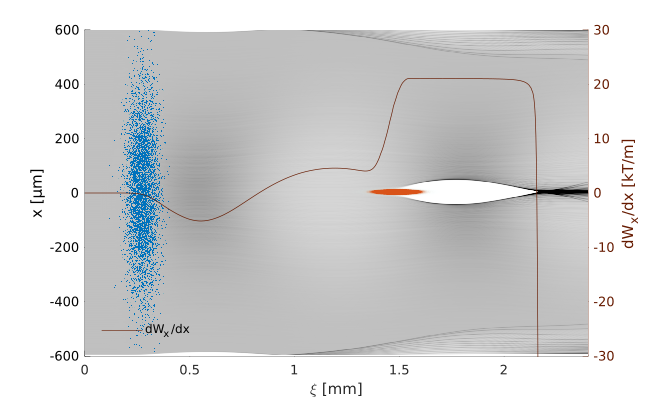
\includegraphics[width=\linewidth,trim={2mm 0mm 2mm 0mm},clip]{figures/plasmaDenTWake}
    \caption{\label{Fig:PlasmaDenTWake} The plasma density in grey with the proton beam (blue) and the electron beam
        (red) superimposed. The line plot indicates the transverse wakefield gradient $dW_{x}/dx$ where
        $W_{x} = E_{x} - v_{b} B_{y}$, evaluated along the beam axis.}
\end{figure}

%~ - describe proton beam wake structure [similar to that of a modulated proton beam] (simulation results to show:
%~   unloaded wake)

The single drive beam setup is designed to behave similarly to the self-modulated case. However, since the drive beam is
prevented from significant transverse evolution, we are presented with an idealised case where the electron witness beam
sees consistent wakefields throughout the plasma stage. The $E_{z}$-field generated by the proton drive beam is seen as
the blue line in figure \ref{Fig:BeamLoading}, shown with and without the electron beam present. With a proton beam
density $n_{pb} \simeq n_{0}$, we are in the quasi-linear regime but near non-linear \cite{rosenzweig:2010}. There is
some depletion of plasma electrons, but not enough to form a bubble. The dashed green line in the lower part of figure
\ref{Fig:BeamLoading} shows that the on-axis plasma density has a depletion of $67\%$, close to what we see in full
scale reference simulations for AWAKE Run 2 \cite{awake_collaboration:2016}.

%~ - by varying the current of the electron beam, the electron beam may load the wake and the longitudinal field can be
%~   flatten and energy spread reduced [well known result, Tzoufras]

The witness beam generates its own wakefield, which in the accelerating phase partially cancels out the $E_{z}$ field
generated by the drive beam. For a finite length beam this causes the particles in the tail of the witness beam to be
accelerated less than those at the front resulting in higher energy spread in exchange for higher energy transfer
\cite{van_der_meer:1985}. Since $E_{z} \propto \rho_{b}$, a beam profile $\rho_{b}(\xi)$ that perfectly flattens the
accelerating field within the witness beam will reduces energy spread to zero. The ideal shape is triangular or
trapezoidal with the peak density in the direction of the beam velocity \cite{katsouleas:1987, tzoufras:2009}.

%~ - the electron beam blows out the remaining plasma electrons. The transverse fields are dominated by the linear
%~   focusing fields originating from the ion background, leading to emittance preservation of the part of the electron
%~   beam inside the bubble [loading of a quasi-linear wake, and still get emittance preservation: this is new]
%~   (simulation results to show: loaded wake, with bubble - many different aspects of this, trans., long. field,
%~   electron densities etc. )

\begin{figure}[hbt]
    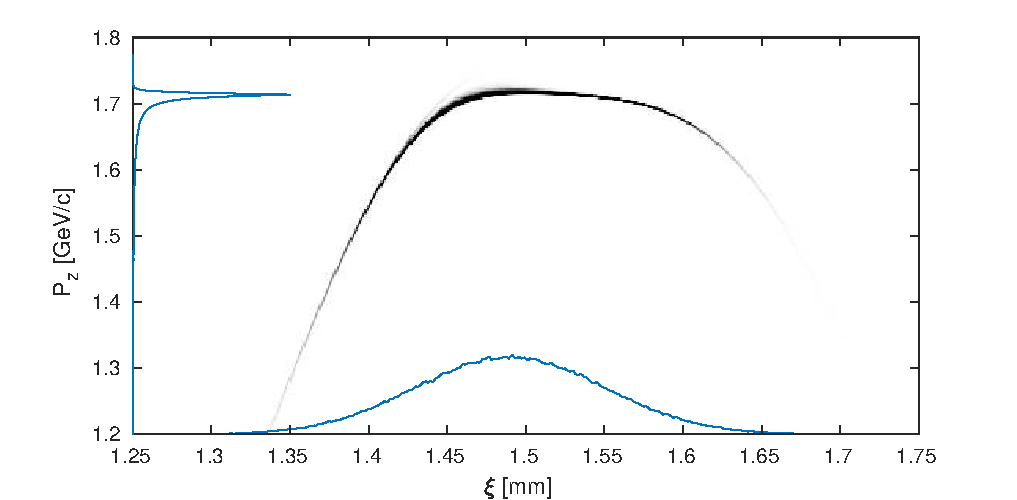
\includegraphics[width=\linewidth,trim={2mm 0mm 2mm 0mm},clip]{figures/beamPhaseSpace}
    \caption{\label{Fig:BeamPS} Phase space charge distribution of a $100\unit{pC}$, $60\unit{\mu m}$ long witness beam
        after $4\unit{m}$ of plasma. Mean momentum is $1.67\unit{GeV/c}$ with an RMS spread of $87\unit{MeV/c}$
        ($5.2\%$) for the full beam.}
\end{figure}

\begin{figure*}[hbt]
    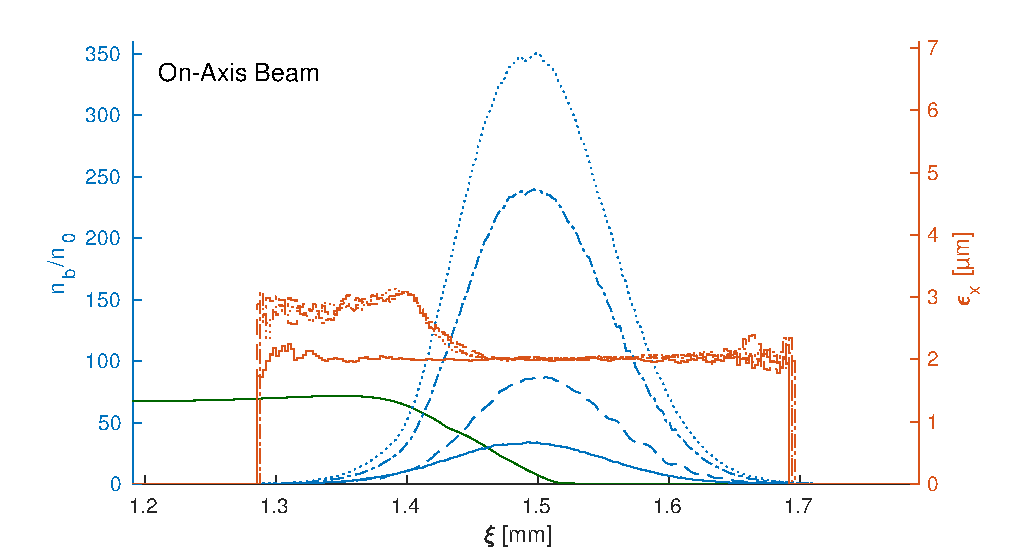
\includegraphics[width=0.495\linewidth,trim={2mm 0mm 2mm 0mm},clip]{figures/beamEmittance}
    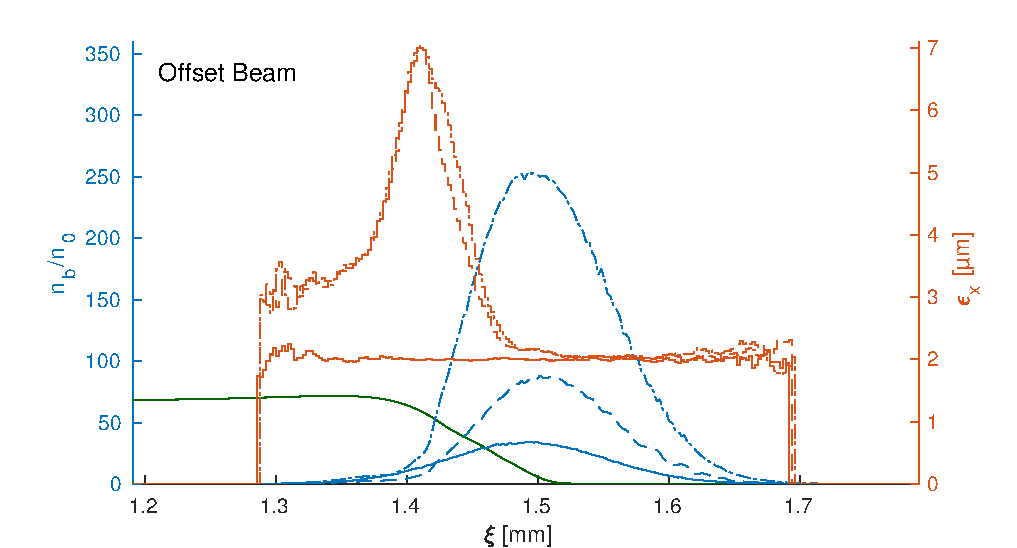
\includegraphics[width=0.495\linewidth,trim={2mm 0mm 2mm 0mm},clip]{figures/beamEmittanceOffset}
    \caption{\label{Fig:BeamEmitt} The red lines show a moving window calculation of transverse normalised emittance for
        an on-axis beam with respect to the drive beam axis (left) and an offset beam (right) with an offset of one
        $\sigma_{x} = 5.24\unit{\mu m}$ in the x plane. The moving window for emittance calculation is longitudinal
        slices of $l = 4\times\Delta\xi = 18.75\unit{\mu m}$ with a $\Delta\xi$ resolution. Only slices with more than
        $100$ macro particles have been included, which accounts for the abrupt edge as well as the noise at either end
        of the beam due to low statistics. The blue lines show the peak electron beam density profile. For reference,
        the plasma density profile is included in green, but scaled up by a factor of $100$ to be visible. The solid
        lines are at the plasma entry point, the dashed lines after $4\unit{m}$ of plasma, the dash-dotted after
        $40\unit{m}$, and the dotted after $100\unit{m}$. In order to sustain a stable accelerating field for the
        witness beam, these simulations were run with an LHC energy drive beam of $7\unit{TeV}$ to avoid de-phasing
        which causes the structure to break down after about $50\unit{m}$.}
\end{figure*}

\begin{figure*}[hbt]
    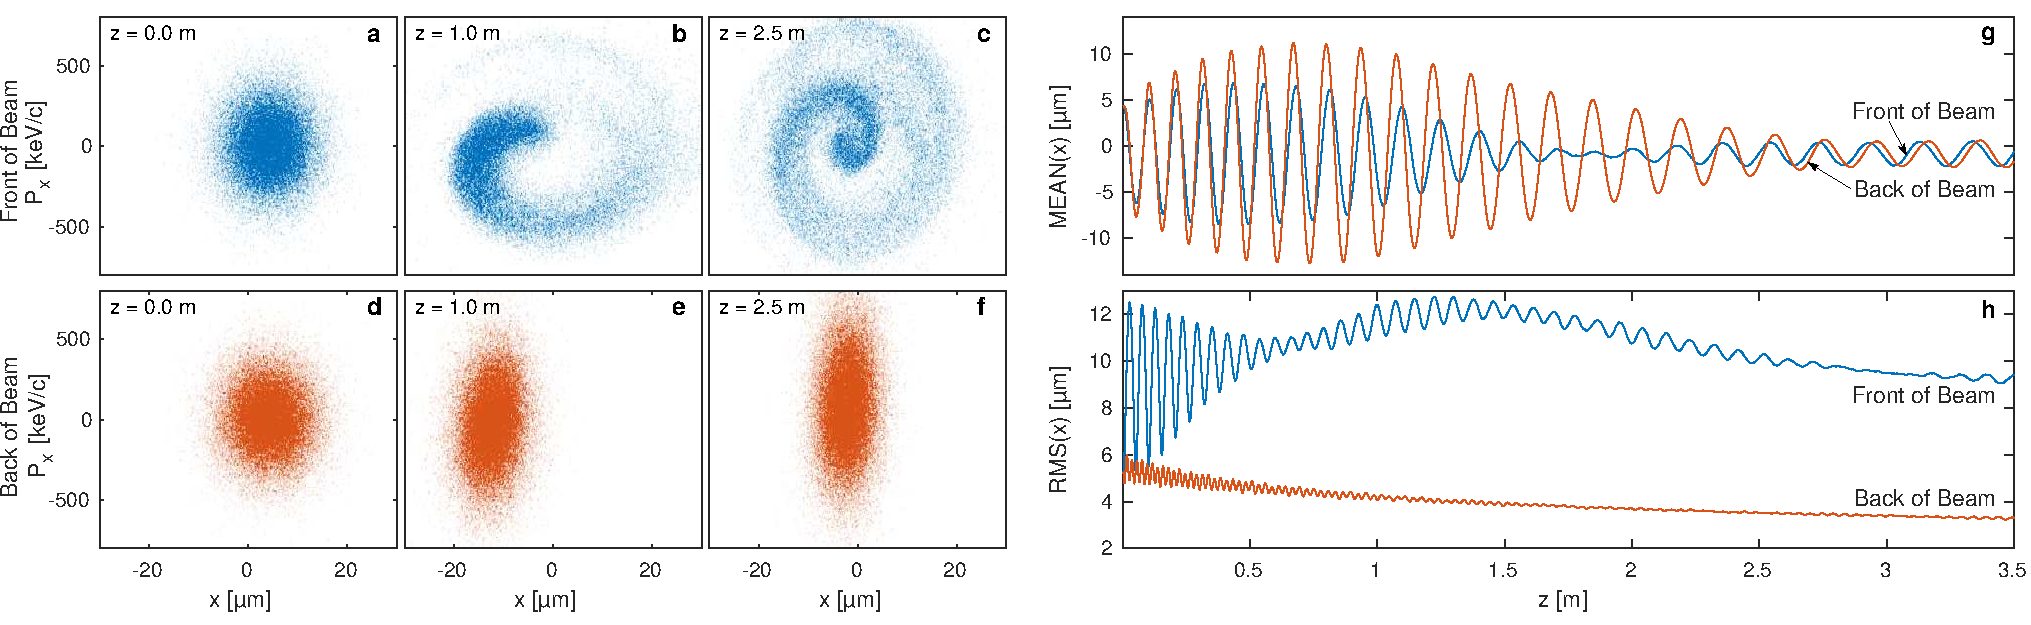
\includegraphics[width=\linewidth,trim={0mm 0mm 0mm 0mm},clip]{figures/beamFilamentationAll}
    %~ 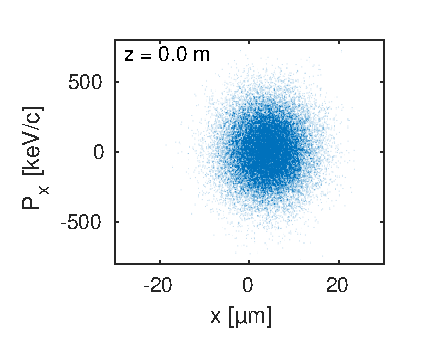
\includegraphics[height=22.2mm,trim={ 0mm 9.5mm  6mm 0mm},clip]{figures/beamFilamentation01}
    %~ 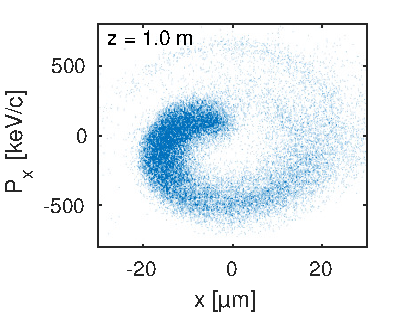
\includegraphics[height=22.2mm,trim={16mm 9.5mm  6mm 0mm},clip]{figures/beamFilamentation02}
    %~ 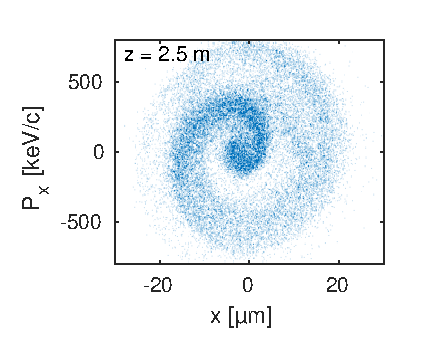
\includegraphics[height=22.2mm,trim={16mm 9.5mm  0mm 0mm},clip]{figures/beamFilamentation03}
    %~ 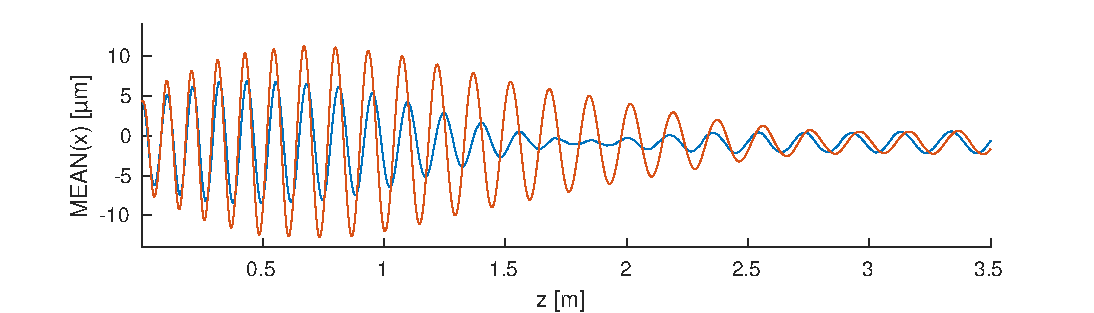
\includegraphics[height=22.2mm,trim={10mm 9.5mm 15mm 0mm},clip]{figures/beamOffsetMean}
    %~ \\
    %~ 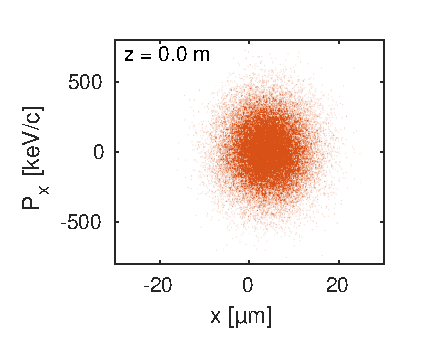
\includegraphics[height=26.0mm,trim={ 0mm 0.1mm  6mm 2mm},clip]{figures/beamFilamentation04}
    %~ 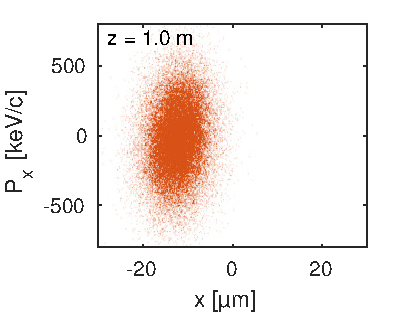
\includegraphics[height=26.0mm,trim={16mm 0.1mm  6mm 2mm},clip]{figures/beamFilamentation05}
    %~ 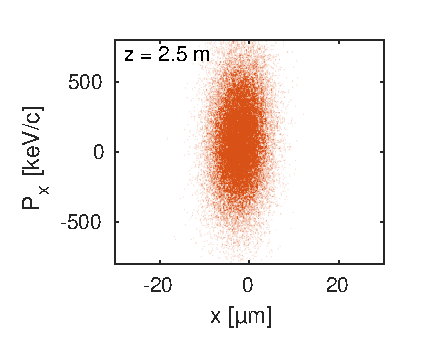
\includegraphics[height=26.0mm,trim={16mm 0.1mm  0mm 2mm},clip]{figures/beamFilamentation06}
    %~ 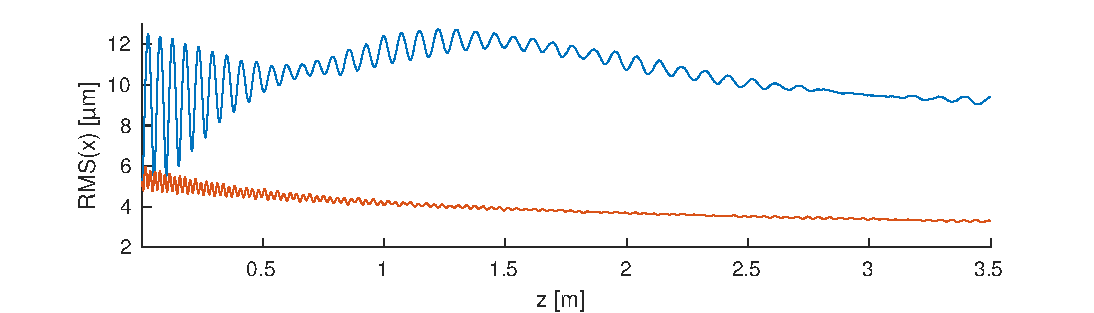
\includegraphics[height=26.0mm,trim={10mm 0.1mm 15mm 2mm},clip]{figures/beamOffsetRMS}
    \caption{\label{Fig:BeamFilament} The left plots show the transverse phase space of the electron beam at different
        plasma positions. The Right side shows the macro particle mean position (top) and RMS spread (bottom). The blue
        particles and lines represent particles with position $1.40\unit{\mu m} < \xi < 1.42\unit{\mu m}$. The red
        particles and lines represent particles with position $1.55\unit{\mu m} < \xi < 1.57\unit{\mu m}$.}
\end{figure*}

For Gaussian beams a reasonable flat field, and consequently low energy spread, can be achieved by controlling the
charge density to achieve a similar effect. This, however, puts the front of the witness beam outside of the ideal
region while the middle bulk of the beam has a trapezoidal-like shape. In our case, with a matched beam to the plasma
density defined by equation \ref{EQ:Matched}, we are limited on how much total charge we can accelerate without reaching
charge densities that will overload the field. The test case shown in figures \ref{Fig:BeamLoading} and
\ref{Fig:PlasmaDenTWake} has a total charge of $100\unit{pC}$ with a $\sigma_{r}=5.23\unit{\mu m}$ matching an initial
normalised emittance $\epsilon_{0} = 2\unit{\mu m}$.

As illustrated in figure \ref{Fig:BeamPS} our base case of a $100\unit{pC}$, $60\unit{\mu m}$ long witness beam, as
expected, shows a difference in energy transfer to the tail of the beam compared to the centre where the $E_{z}$-field
is nearly flat. Also the front of the beam has a large tail in momentum space as this regions sees a consistently
smaller accelerating field. The positioning of the witness beam is chosen to put the bulk of the charge as close to the
peak accelerating field as possible.

Due to the high charge density resulting from a very narrow beam, the witness beam's own wakefield reaches the full
non-linear regime with $n_{eb} \approx 35\times n_{0}$. This second wakefield is driven by the beam's own front. The
space charge rapidly becomes high enough to start expel plasma electrons from the beam axis, and form the characteristic
electrons sheet that defines the blowout regime. As a result the plasma region reaches full depletion close to the peak
of the electron beam, which in turn generates strong focusing fields, with gradients of $20\unit{kT/m}$ near the beam
axis (see figure \ref{Fig:PlasmaDenTWake}).

%~ - the acceleration and the transverse emittance stable on long timescales (simulation results to show: transverse and
%~   longitudinal phase spaces, space long simulation)

The witness beam's self-generated bubble prevents the tailing end of the beam to see any significant emittance growth.
For the majority of the cases we studied that maintained a stable accelerating structure, about $70-80\%$ of the beam
retained its initial emittance. Figure \ref{Fig:BeamEmitt} shows the $100\unit{pC}$ and $\sigma_{z} = 60\unit{\mu m}$
case extended to a $100\unit{m}$ plasma and the drive beam energy increased to $7\unit{TeV}$ (LHC energy) to prevent
de-phasing. De-phasing for the SPS beam case starts to become significant after about $50\unit{m}$.

The on-axis density of the electron beam increases as its gamma factor increases and its transverse size decreases. The
beam radius follows the evolution given by equation \ref{EQ:Matched} with $\lambda_{pe} = \lambda_{0}$ for the section
of the beam where normalised emittance is preserved. This has the potential to cause overloading of the field. However,
our $100\unit{pC}$ case is slightly under loaded, and this does not seem to be a significant effect in this instance.

%~ - in this regime, emittance preservation is robustness to drive-witness offset [this is new] (simulation results to
%~   show: transverse and longitudinal phase spaces, long offset simulation)

Our configuration also shows some robustness to small electron beam transverse offsets as the bubble generated by the
witness beam wakefield follows the beam itself. The head of the beam does not benefit from this effect, and we see
some defocusing in this region. This effect is likely to be greater for larger offsets as the beam oscillates around
the axis of the drive beam wakefield (see right hand plots of figure \ref{Fig:BeamFilament}). However, since the proton
wakefield creates a quasi linear condition, we still see the head of the beam stabilising after some time. The off-axis
case has a larger initial emittance growth (see left hand plots of figure \ref{Fig:BeamFilament}), but the growth levels
off after the first few metres and stays constant for the remainder of the plasma accelerator section (figure
\ref{Fig:BeamEmitt}).

% ******************************************************************************************************************** %
\section[\label{S:PO}]{Parameter Optimisation}
%~ Sec N+1: Parameter optimization, or, parameter scaling [in this section we describe how to optimize the electron
%~ beam, and preferably some scalings]
%~ - how to select electron beam parameters:
%~ - longitudinal parameters bunch length and current (simulations results to show: overloaded/underloaded cases)
%~ - transverse parameters of electron emittance / matching [too large, outside bubble.  Do we see increased head
%~   erosion -> faster decay]?  (simulations results to show: evolution of high emittance vs low emittance cases)
%~ (- plasma density?)
% ******************************************************************************************************************** %

\begin{figure}[hbt]
    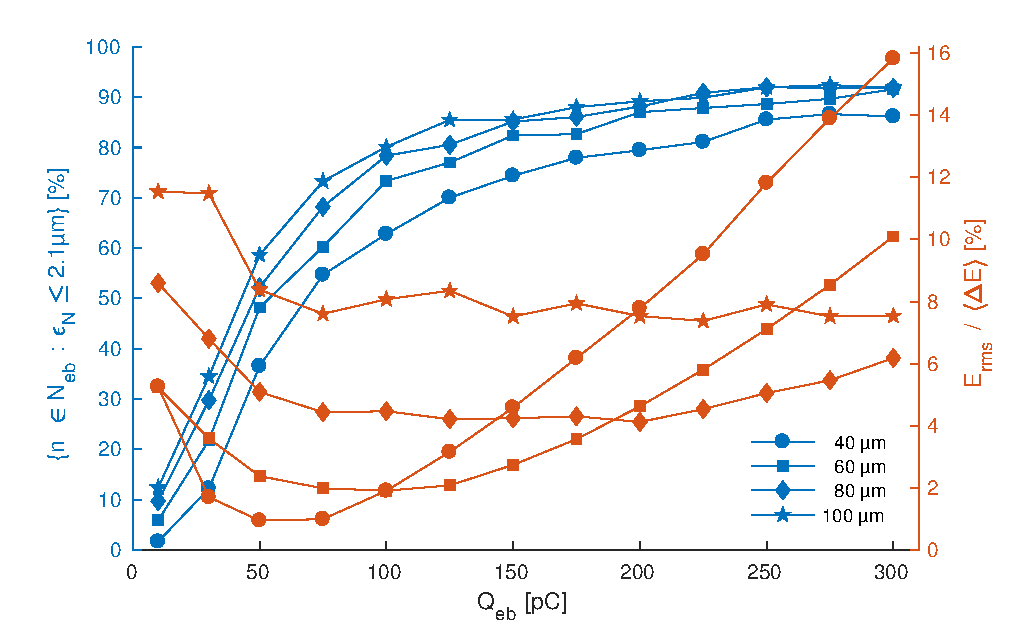
\includegraphics[width=\linewidth,trim={2mm 0mm 2mm 0mm},clip]{figures/beamQuality}
    \caption{\label{Fig:BeamQ} Ratio of total beam charge with an emittance growth $\Delta\epsilon \leq 5\%$ as a
        function of initial beam charge (blue), and relative energy spread (red), after $4\unit{m}$ of plasma and with
        an initial emittance $\epsilon_{N,0}=2\unit{\mu m}$. These are shown for four different $\sigma_{z}$ from
        $40\unit{\mu m}$ to $100\unit{\mu m}$. The detailed studies presented in beam loading section corrspond to the
        square marked lines at $100\unit{pC}$.}
\end{figure}

\begin{figure}[hbt]
    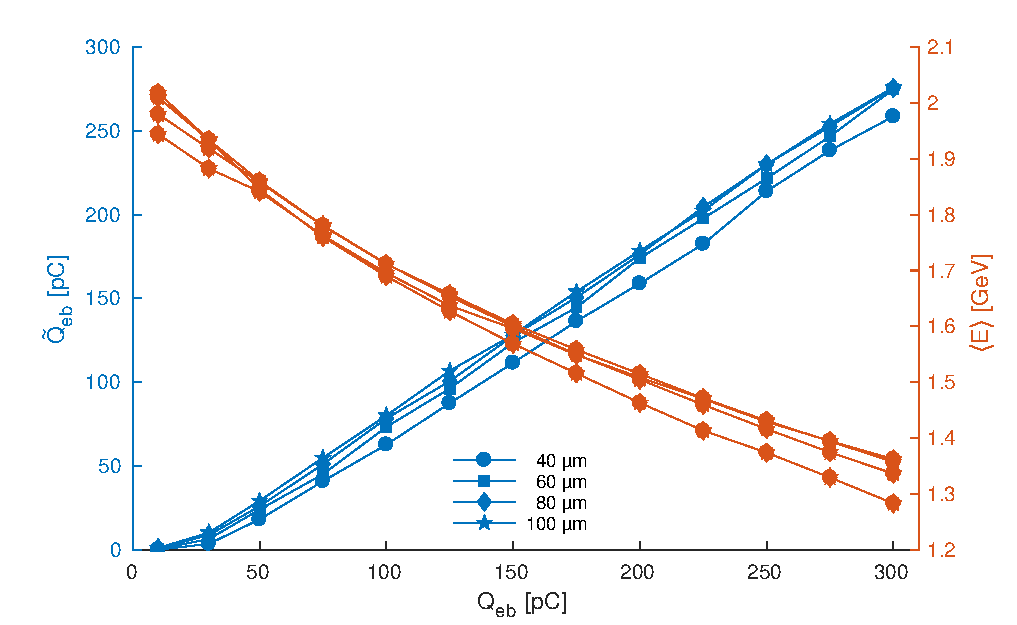
\includegraphics[width=\linewidth,trim={2mm 0mm 2mm 0mm},clip]{figures/beamQualityAbs}
    \caption{\label{Fig:BeamQAbs} Total beam charge with an emittance growth $\Delta\epsilon \leq 5\%$ as a function of
        initial beam charge (blue), and final momentum (red), after $4\unit{m}$ of plasma and with an initial emittance
        $\epsilon_{N,0}=2\unit{\mu m}$.}
\end{figure}

For accelerator applications in general, and also for Run 2 of the AWAKE experiment, it is desirable to maximise the
charge that can be successfully accelerated in the witness beam. However, a longitudinally constant accelerating
field depends on both the position and the charge density of the witness beam \cite{katsouleas:1987, tzoufras:2009}.

The large number of parameters involved makes the problem difficult to solve in simulations, and difficult to measure in
experiments. Presented in figures \ref{Fig:BeamQ} and \ref{Fig:BeamQAbs} is a parameter scan for a matched beam with
initial normalised emittance $\epsilon_{N,0}=2\unit{\mu m}$ after propagating through $4\unit{m}$ of plasma. We ran the
scan with beam charge from $10\unit{pC}$ to $300\unit{pC}$ and with length $\sigma_{z}$ from $40\unit{\mu m}$ to
$100\unit{\mu m}$. We see from figure \ref{Fig:BeamQ} that both the $40\unit{\mu m}$ and the $60\unit{\mu m}$ beam has a
well defined minimum energy spread with a beam charge $\geq 50\unit{pC}$ and $\approx 100\unit{pC}$ respectively. Lower
beam charges tend to underload the field, while higher beam charges tend to overload. It is also clear that long beams
with respect to the accelerating flank of the $E_{z}$-field, $\approx\lambda_{pe}/4$, will not optimally load the field
along its length thus experiencing a larger spread in energy.

A higher charge beam will generate a non-linear wakefield closer to the head of the beam, which in turns ensures that a
smaller portion of the beam experiences the quasi-linear region with emittance growth. As figure \ref{Fig:BeamQAbs}
illustrates, a higher charge also results in a lower energy gain.

% ******************************************************************************************************************** %
\section[\label{S:D}]{Discussion}
% discussion of optimal electron beam parameters
% implications for AWAKE Run 2
% ******************************************************************************************************************** %


% ******************************************************************************************************************** %
\section[\label{S:C}]{Conclusion}
% ******************************************************************************************************************** %

\section[\label{Ack}]{Acknowledgements}
% ******************************************************************************************************************** %

The simulations for this study have been run using the open source version of QuickPIC released in early 2017 and owned
by UCLA.

These numerical simulations have been made possible through access to the Abel computing cluster in Oslo, Norway. Abel
is maintained by UNINETT Sigma2 AS and financed by the Research Council of Norway, the University of Bergen, the
University of Oslo, the University of Tromsø and the Norwegian University of Science and Technology. Project code:
nn9303k. Some of the simulations were also run on the student-maintained computing cluster ``Smaug'' at the University
of Oslo, Department of Physics.

The authors would also like to acknowledge the OSIRIS Consortium for providing access to the OSIRIS framework. OSIRIS
was used extensively for simulations leading up to the work presented in this paper.

% ******************************************************************************************************************** %
\bibliography{Bibliography}
\end{document}
% ******************************************************************************************************************** %
